\documentclass[UTF8,a4paper]{paper}
\usepackage{ctex}
\usepackage{amsmath}
\usepackage{graphicx}
\usepackage{wrapfig}
\title{
\begin{large}电子技术课程设计——基于无人车的场地探测和3D重建系统\end{large}\\
预习报告
}
\author{
    张蔚桐\ 2015011493\ 自55\\
    陈崴\ \ \ \ 2015011481\ 自55}
\begin {document}
\newcommand{\tabincell}[2]{\begin{tabular}{@{}#1@{}}#2\end{tabular}}
\maketitle
\tableofcontents    
\clearpage
\section{选题背景及课题简介}

\section{方案比较与选择}
\subsection{主控元件的选择}
首先我们考虑主控元件的选择,根据我们的技术水平和课题的情况,可供选择的主控芯片为MCU
(单片机)和FPGA。相比FPGA,MCU具有开发相对简单的优势,以串口通信协议为例,大部分MCU
的系统库中均已经封装了串口通信协议,然而FPGA相对更接近底层,因此需要自行完成相关的通信协议
的封装,这将消耗大量的时间和精力。

然而,相比于MCU,FPGA在速度和并行性方面有着很大的优势。根据我们查阅的资料,以STMF103为例,
其时钟速度可以达到72MHz,然而由于串行执行的原因,IO速度相对于FPGA较低;对比我们使用的Xilinx
FPGA,其时钟速度可以达到100MHz,同时高度并行使得模块之间互相不干扰,保证了IO速度等要求。

因此,考虑到性能要求以及课程需要,我们在硬件方面采用了FPGA作为主控进行开发。
\subsection{通信机制的选择}
根据查阅的资料,可供选择的无线通信机制有如下两种

\begin{enumerate}
    \item WiFi信道

    这种通信机制需要将WiFi模块植入硬件,使得小车可以联网传输信息。
    上位机或移动平台使用WiFi下载信息。这种方式的优势一方面是信息传输距离较远,
    在一个路由器覆盖的范围内,信息均可以被传输。另一方面可拓展性也比较强,
    如果设计了合理的联网方式,将进一步解除距离限制,通过将信息上传到云空间,
    用户可以在任何联网的地区完成信息的收取和对小车的控制。

    这种通信机制的缺点是过于复杂,尤其是使用FPGA进行开发的情况下,网络通信协议
    将带来更大的开发时间消耗,不适用于本课程的短期开发。

    \item 蓝牙信道

    这种通信机制利用蓝牙模块,蓝牙模块已经将蓝牙信道封装成串口的形式,
    从很大程度上方便了开发。同时,通过对电脑,移动设备上的蓝牙模块进行开发,
    用户可以不依赖于第三方设备(如路由器)和小车进行通信。通信速度上相比WiFi也
    更快,但相比而言缺点是通信距离受到明显限制。
\end{enumerate}
综合两种通信机制的优缺点,我们选择蓝牙信道作为通信手段。
\subsection{供电方式的选择}
首先通过查阅可能使用到的外设的技术手册,我们大概确定了供电需求为
\begin{itemize}
    \item 5V@1.5A
    \item 3.3V@1.5A
    \item 9V@40A
\end{itemize}
其中5V@1.5A负责向FPGA 5V@1A供电,3.3V电源负责向外设供电,例如我们采用的摄像头OV7670
采用的供电电压为3.3V@100mA。9V@40A电源负责向电机供电,并应接受PWM调制来控制电机转速。

通过查阅资料我们发现,供电的难点在9V40A电源,而5V@1.5A电源和3.3V@1.5A电源
均可以使用实验室提供的TPS54160SMT芯片完成设计。9V40A电源的电流限额主要受到电机供电电流要求
影响,如图\ref{fig1}所示,电机的空载电流2.4A,最高效率电流11A,堵转电流52.8A,根据网上
查阅的相关资料,电机的限流应当是最高效率电流的约4倍,因此设计9V@40A电源负责向电机供电。

这里讨论9V@40A电源的设计问题。因为需要接受PWM信号调制,因此我们采用了H桥进行设计。

%这里介绍H桥

通过搜索符合要求的元件,我们发现合理的解决方案为bts7960/7961芯片和自行搭建H桥两种方案

bts7960/7961芯片是接受5VPWM信号调制的,输入电压5.5V至27V@43A的半H桥电路,
采用SMT封装,输出电流符合要求。
然而,由于我们电机的最高输入电压为9V,而电源电压约为14V,因此PWM信号的占空比不可过高,
因此我们考虑采用这种设计的基础上在bts输出管脚加对地限压保护,
保证输出电压不超过电机的最高电压限制。

而自行搭建H桥,因为工艺比较复杂,同时在网上找不到合适的大功率MOS管供应商,
因此我们放弃了这个方案。

回顾整个供电系统的设计,我们可以采用SMT技术来完成PCB版的设计工作,这从很大程度上减小了
PCB版面积的大小,方便了进一步的开发。

\subsection{摄像头数据传输技术的选择}
我们采用的OV7670摄像头,可以输出25fps 640*480 VGA格式的RGB三色图像,输出采用8线同步并行传送
因此输出时钟速度可以达到$25*640*480 \approx 8\mathrm{MHz}$。
收到蓝牙信道是串行接口的原因,蓝牙信道的速度必须达到8MB/s,这是一般蓝牙系统很难做到的。
因此不论是FPGA读取信息还是蓝牙传输信息的速度,均不如摄像头采集数据的速度,需要找到合理的解决方式。

经过我们查阅相关资料发现,OV7670的传输方式有如下三种形式
\begin{wrapfigure}{r}{0pt}
        \centering
        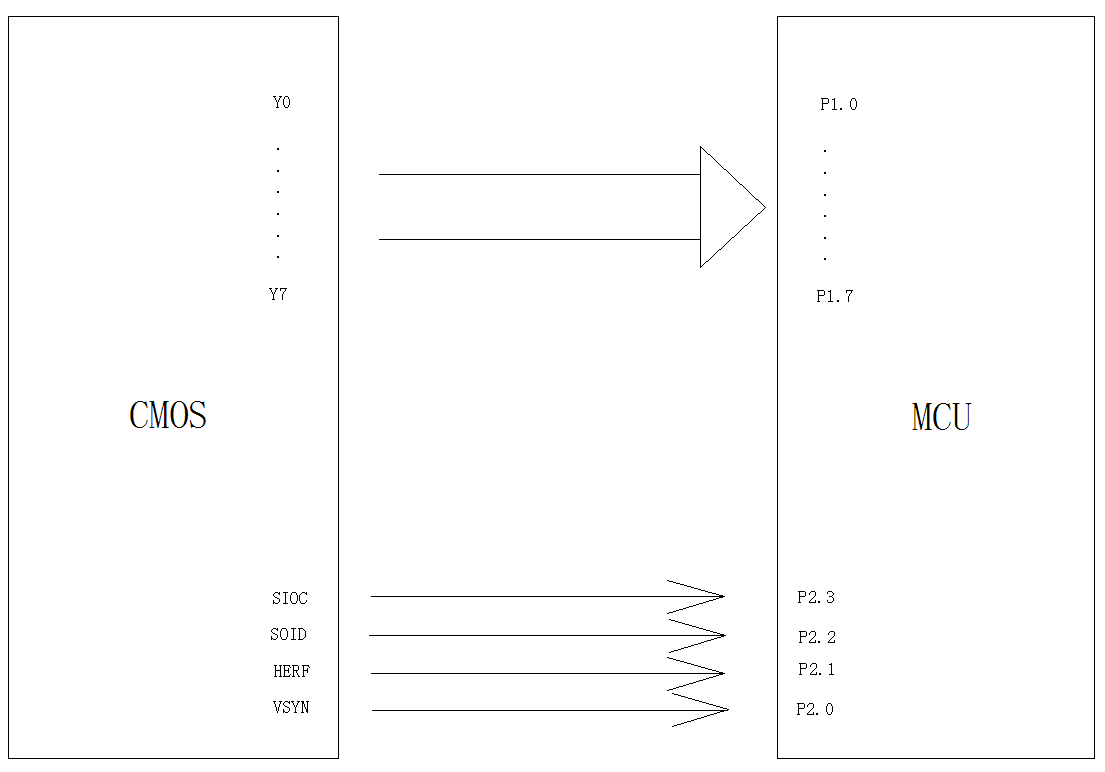
\includegraphics[width=60mm]{NFIFO.png}
        \caption{MCU/FPGA直接采集}
        \label{fig2}
        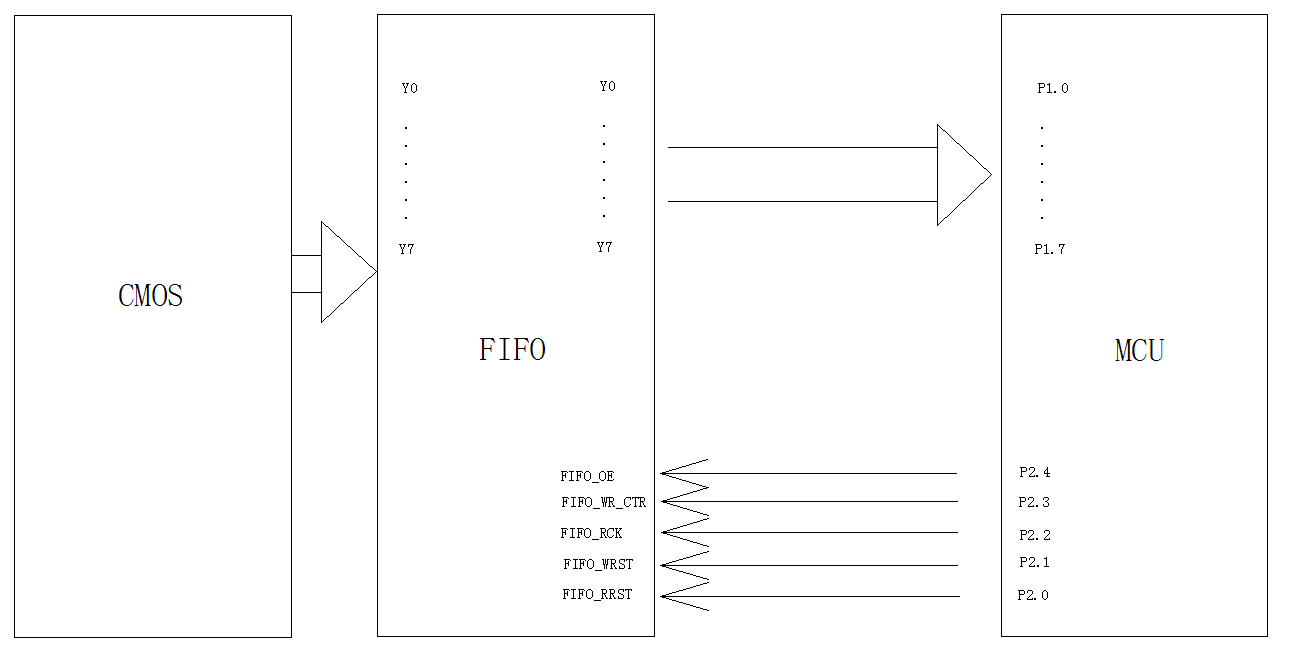
\includegraphics[width=60mm]{FIFO.png}
        \caption{FIFO采集}
        \label{fig3}
    \end{wrapfigure}
\begin{itemize}
    \item MCU/FPGA直接采集:

    如图\ref{fig2}所示,这种方法是最简单,最直接,但也是最不好实现的方法,
    以MCU为例,多数的CMOS 芯片(如ov7670)的时钟速度可高达24M,
    一般MCU的IO 端口速度根本不可能达到,所以需要高速MCU。
    这对多数用户来讲有些不现实。但也不是完全没有办法在低速上实现采集,
    方法也很简单,那么就是降低CMOS 的输出速度,
    不过这需要靠外部的晶振和内部的PLL 电路以及像素时钟速度,
    帧速等多个寄存器共同设置,并且要和MCU 的IO 速度匹配才可实现。
    但这么做将带来巨大的寄存器设置工作量并导致硬件图像的采集速度
    可能下降到0.5 帧以下,同时带来图像失真的可能。
\end{itemize} 

\begin{itemize}
    \item DMA方式

    这种方式主要用于MCU中,FPGA中这种方式效果不明显,DMA控制器使得数据
    可以绕过CPU直接进入内存,但是在FPGA中,同时受到串口通信速度的影响,
    这种方式效果也不是很明显

    \item FIFO模块采集

    如图\ref{fig3},用户只需要按上述时序图控制相关的几个控制引脚即可,可以很
    方便的使用在低速MCU上,另外一个好处是,可以直接IO 口读取数据,
    读出的数据可以直接送屏,也可以经过MCU 简单处理;当然也可以不经过
    MCU,直接送到屏等外围器件使用。对于FPGA,以及速度相对较低的串口单元,
    使用FIFO也能很大程度的解决速度不同步的问题。

\end{itemize}
\subsection{车辆位置角度信息处理方式的选择}
为了进一步增强3D建模的精度,我们希望能够采集车辆的位置信息和角度信息。
由于摄像头和车辆是相对固定的,这样也就获得了摄像头的位置信息和角度信息。

根据我们查阅到的资料,车辆的位置信息和角度信息有几种不同的获取方式,如下所示。
\begin{itemize}
    \item 惯性测量单元(IMU)模块

    通过加速度计和陀螺仪的信息,可以直接读取车辆的加速度和角度。
    经过积分之后可以得到车辆的速度信息和角度信息,这种方法最简单,
    但是误差最大,加速度计易受到颠簸,碰撞,刹车等造成的脉冲影响,
    并进一步影响积分的准确性。角速度计(陀螺仪)具有一般性的零点迁移
    问题,这包括动态的零点波动和静态的温漂。经过积分会导致角度信息
    相当不准确。这种方法只能作为一种简单的参考,实用时必须加以处理。

    \item 磁场计

    通过对地磁角度的测定,可以直接获取车辆的角度,并通过加速度计等
    方式获得车辆的速度,这种方式误差相对前一种较小,
    但是受外界磁场的影响比较严重,尤其是当存在10A绕组的电机驱动时,
    这种方法可以认为无效。

    \item 码盘

    这种方法通过测量车辆四轮的转速经过解算得到车辆的具体位置,相比于
    之前几种方式,这种方式依赖于更加准确的光电传感器,因此得到的值也
    相对比较准确,这种方法的难点在于必须对车辆的刚性模型进行建模,
    同时安装码盘也是一个硬件上的难点。
\end{itemize}
综合提到的几种方法,我们计划采取IMU+信号处理+码盘解算几种方式
得到车辆的具体位置,希望通过反馈等方式可以得到更准确的车辆控制。
\section{基于FPGA的数字系统框图}
\section{传感器/执行机构接口电路图}
\section{基于Webench的电源电路仿真}
\end{document}